\documentclass{article}

\usepackage{graphicx}
\usepackage{tikz}
\usepackage{tikzsymbols}
\usetikzlibrary{calc,patterns,shapes.geometric}
\pagestyle{empty}
\usepackage[margin=0pt]{geometry}
\geometry{papersize={14in,12in}}

\def\centerarc[#1](#2)(#3:#4:#5){\draw[#1] ($(#2)+({#5*cos(#3)},{#5*sin(#3)})$) arc (#3:#4:#5);}

\begin{document}
	\begin{figure}
		\centering
		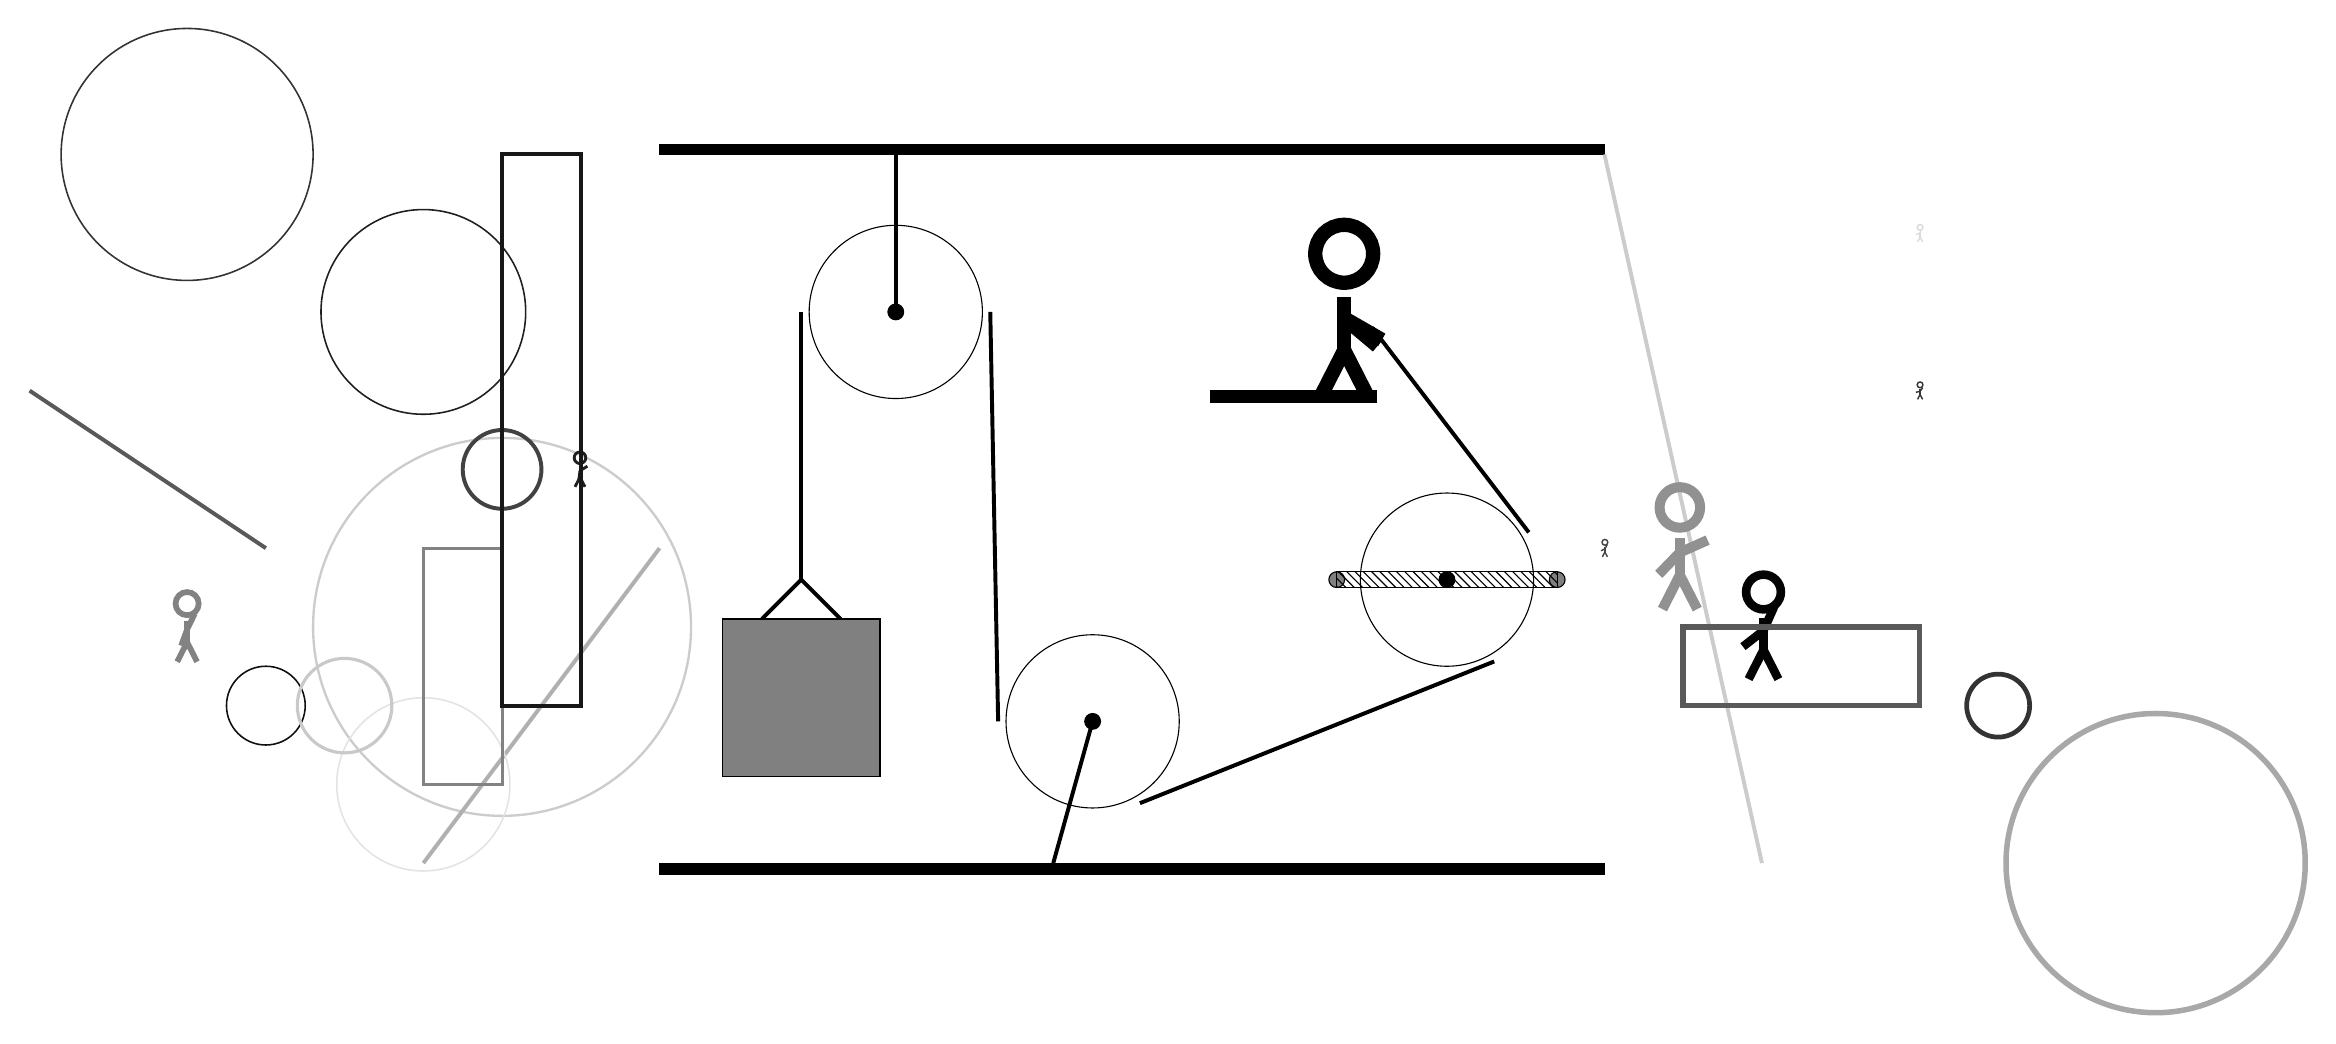
\begin{tikzpicture}
			%%%%% START %%%%%
			
			\draw[fill=black] (-2, 9) rectangle (10, 9.125);
			
			\draw (1, 7) circle (1.1);
			\draw[fill=black] (1, 7) circle (0.1);
			\draw[line width=0.5mm] (1, 9) -- (1, 7);
			
			\draw[line width=0.5mm, color=black!65](-7, 4) -- (-10, 6);
			
			\draw [line width=0.7mm, color=black!34](17, 0) circle (1.9);
			\draw [line width=0.3mm, color=black!20](-4, 3) circle (2.4);
			\draw[line width=0.5mm, color=black!31](-5, 0) -- (-2, 4);
			
			\node[line width=0.4mm, color=black!73] at (10, 4) {\Strichmaxerl[1][28][60]};
			\draw [line width=0.2mm, color=black!80](-8, 9) circle (1.6);
			\draw [line width=0.6mm, color=black!80](15, 2) circle (0.4);
			
			\draw [line width=0.2mm, color=black!11](-5, 1) circle (1.1);
			\draw[line width=0.2mm, color=black!14] (-3, 3) rectangle (-3, 8);
			
			\draw [line width=0.5mm, color=black!74](-4, 5) circle (0.5);
			
			\draw [line width=0.2mm, color=black!94](-7, 2) circle (0.5);
			\draw[line width=0.5mm, color=black!20](10, 9) -- (12, 0);
			\draw [line width=0.2mm, color=black!88](-5, 7) circle (1.3);
			\node[line width=0.7mm, color=black!14] at (14, 8) {\Strichmaxerl[1][3][79]};
			\draw[line width=0.4mm, color=black!49] (-4, 4) rectangle (-5, 1);
			\node[line width=0.5mm, color=black!99] at (12, 3) {\Strichmaxerl[6][38][66]};
			
			\node[line width=0.7mm, color=black!88] at (-3, 5) {\Strichmaxerl[2][83][31]};
			\draw [line width=0.4mm, color=black!21](-6, 2) circle (0.6);
			\node[line width=0.4mm, color=black!79] at (14, 6) {\Strichmaxerl[1][14][53]};
			\node[line width=0.6mm, color=black!43] at (11, 4) {\Strichmaxerl[7][46][24]};
			\node[line width=0.5mm, color=black!49] at (-8, 3) {\Strichmaxerl[4][70][64]};
			
			\draw[line width=0.5mm, color=black!91] (-3, 9) rectangle (-4, 2);
			\draw[line width=0.7mm, color=black!65] (11, 2) rectangle (14, 3);
			
			\draw (3.5, 1.8) circle (1.1);
			\draw[fill=black] (3.5, 1.8) circle (0.1);
			\draw[line width=0.5mm] (3.5, 1.8) -- (3.0, 0);
			
			\draw[fill=white](8, 3.6) circle (1.1);
			\draw[fill=black] (8, 3.6) circle (0.1);
			\draw[fill=black!50] (9.4, 3.6) circle (0.1);
			\draw[fill=black!50] (6.6, 3.6) circle (0.1);
			\draw[pattern=north west lines, pattern color=black] (6.6, 3.7) rectangle (9.4, 3.5);
			
			\draw[line width=0.5mm](-0.7, 3.1) --  (-0.2, 3.6) -- (0.3, 3.1);
			\draw[fill=black!50] (-1.2, 3.1) rectangle (0.8, 1.1);
			
			\draw[line width=0.5mm](-0.2, 7) -- (-0.2, 3.6);
			\centerarc[line width=0.5mm](1, 7)(180:0:1.2000000000000002)
			\draw[line width=0.5mm](2.2, 7) -- (2.3, 1.8);
			\centerarc[line width=0.5mm](3.5, 1.8)(180:300:1.2000000000000002);
			\draw[line width=0.5mm](4.1, 0.7608) -- (8.6, 2.5608);
			\centerarc[line width=0.5mm](8, 3.6)(300:390:1.2000000000000002);
			\draw[line width=0.5mm](9.0392, 4.2) -- (7.05, 6.8);
			
			\node at (6.75, 7) {\Strichmaxerl[10][-220][-30]};
			\draw[fill=black] (5, 6) rectangle (7.1, 5.85);
			
			\draw[fill=black] (-2, 0) rectangle (10, -0.15);
			
			%%%%% END %%%%%
		\end{tikzpicture}
	\end{figure}	
\end{document}